% Document settings

% Common
\DocumentMetadata{pdfversion=1.7, pdfstandard=A-2u}
\documentclass[11pt,letterpaper]{article}
\usepackage{fancyhdr}
\usepackage[]{fncychap}
\usepackage{etoolbox} % patch stuff
\usepackage[margin=1in]{geometry}
\usepackage{multirow}
\usepackage{longtable,booktabs, array, threeparttable} % typesetting
\usepackage{bookmark}
\usepackage[acronym]{glossaries-extra}
\pagestyle{plain}
\usepackage{parskip, setspace}

% Plots and Color
\usepackage{graphicx}
\graphicspath{{images/}{drawings/}}
\usepackage[font=footnotesize,labelfont=bf]{caption}
\usepackage{xcolor,colorspace}
\usepackage{tcolorbox}
\usepackage{pgfplots}
\pgfplotsset{compat=newest}
\usepackage{epstopdf}
\usepackage[american voltages]{circuitikz}


% Math stuff
\usepackage{mathtools} % loads amsmath and fixes its bugs, empheq, etc
\usepackage{amssymb}
\usepackage{sympytex}
\usepackage{siunitx}
\sisetup{detect-all=true}   % ensure proper font weight
\DeclareSIPrefix\micro{\ensuremath{\symup{\mu}}}{-6} % ensure upright mu for micro
\sisetup{per-mode = repeated-symbol}    % ensure "/" unit delineator
\sisetup{range-phrase = {\text{~to~}}}  % SI range clarity (NIST 811 Ch7.7)
\DeclareMathSymbol{\varOmega}{\mathalpha}{operators}{"0A}   % upright omega for ohms
\providecommand*{\upOmega}{\varOmega}   % upright Ohms
\DeclareSIUnit{\sq}{\ensuremath{\Box}}    % sheet resistance
\DeclareSIUnit{\Siemens}{S}
\DeclareSIUnit{\torr}{Torr} % add torr to siunitix 3
\DeclareSIUnit\sig{\ensuremath{\sigma}}
\DeclareSIUnit\ppm{ppm}
\usepackage{nicefrac}

% Font
\usepackage{fontspec}
\setmainfont{STIXTwoText}[
	Extension		= .otf,
	UprightFont		= *-Medium,
	BoldFont		= *-Bold.otf,
	ItalicFont		= *-MediumItalic.otf,
	BoldItalicFont 	= *-BoldItalic.otf
    ]
\setmonofont{Fira Code}[
	Extension		= .ttf,
	UprightFont 	= *-Regular,
	Numbers 		= SlashedZero,
	StylisticSet	= {2,5,3,9},
	CharacterVariant= {20,26,30},
  	Contextuals=Alternate
	]
\usepackage[warnings-off={mathtools-colon,mathtools-overbracket},math-style=ISO]{unicode-math}
\setmathfont{STIXTwoMath-Regular.otf} % for symbols
% \usepackage{microtype}
% \UseMicrotypeSet[protrusion]{basicmath} % disable protrusion for tt fonts
\urlstyle{same}

\usepackage[normalem]{ulem} % Enable normal \ul underline
\usepackage{fancyvrb}

\RequirePackage[type={CC},modifier={by-nc-nd},version={4.0},lang={english}]{doclicense}

\usepackage{datetime2} % to satisfy the "\today" in \hypersetup
\DTMusemodule{english}{en-US}
\usepackage{hyperref}
\hypersetup{
    hyperindex=true,
    colorlinks=true,
	bookmarksnumbered,
    bookmarksopen=true,
    linkcolor=blue,
    filecolor=magenta,      
    urlcolor=cyan,
%%%%%%%%%%%%%%%% METADATA %%%%%%%%%%%%%%%%%%%%	
    pdftitle={EE726 Project 5},
	pdfsubject={3.3V Bandgap-Regulated Charge Pump Power Supply for Portable Applications},
    pdfauthor={Chris Biancone},
	pdfpublisher={Chris Biancone},
	pdfkeywords={Regulated Charge Pump; Portable},
%%%%%%%%%%%%%%%%%%%%%%%%%%%%%%%%%%%%%%%%%%%%%%
	pdfproducer=luaLaTeX-1.18.0,
	pdfdate=\today,
	pdflang={en},pdfmetalang={en},
	pdflicenseurl={},
    % pdfpagemode=FullScreen,
}
\usepackage[noabbrev,capitalize]{cleveref}
% this is necessary for IEEEtranDOI.bst to work with hyperkinked DOIs
\newcommand*{\doi}{}
\makeatletter
\newcommand{\doi@}[1]{\href{https://doi.org/#1}{#1}}
\DeclareRobustCommand{\doi}{\hyper@normalise\doi@}
\makeatother

% % % % % % % % % % % Header footer
% % % % % % % % % % %EDIT THIS % % % % % % % % % % % % % % % % % % % %
\pagestyle{fancy}
\fancyhf{}
\lhead{Tech Memo:  Project 5}
\rhead{Chris Biancone}
\lfoot{EE726}
\cfoot{\today }
\rfoot{Page \thepage}
% % % % % % % % % % % % % % % % % % % % % % % % % % % % % % % % % % % % %

% Scale images if necessary, so that they will not overflow the page
% margins by default, and it is still possible to overwrite the defaults
% using explicit options in \includegraphics[width, height, ...]{}
%\setkeys{Gin}{width=\maxwidth,height=\maxheight,keepaspectratio}

% No paragraph indent
\setlength\parindent{0pt}

\begin{document}

\VerbatimFootnotes % allows verbatim text in footnotes

\numberwithin{equation}{subsection}
\numberwithin{figure}{subsection}

	\hspace{4.5in}
	
\includegraphics[width=2in,trim=0cm 0in 0in 0.0in,clip]{images/COE_EME_1505C_hor_k1.pdf}
\newline

\Huge\textbf{EEEE 726: Project 5 \\3.3V Bandgap-Regulated Charge Pump Power Supply for Portable Applications}\\

\Large
\textbf{From:} Chris Biancone \\
\textbf{To: } Dr. Mark Pude \\
\textbf{Date: } \today \\
\textbf{Subject: } Project 5\\
\vspace{0.5in}

\section*{Abstract}
\normalsize
This report presents the design of a regulated charge pump for battery powered portable applications using 3.3V digital logic, typically supplied by 2 series alkaline batteries. The regulation of the charge pump is designed to keep the output voltage within \qty{10}{\%} as the battery discharges down toward \qty{2}{\V}. While this exercise is more of a thought experiment, it worked on the first simulation using Cadence gpdk045\_v5.0 components without verifying the circuit behaviorally and performing limited ``napkin math'' for device sizing.


\section{Design}

This SAR ADC is constructed to meet the requirements specified in \cref{tab:design_req}. Since the comparator is dynamic, the reference current is not used. A typical temperature corner of \qty{40}{\degree\C} is assumed --- simulations at \qty{27}{\degree\C} are not run for this design to save simulation time, since the temperature experienced within an IC would most often be warmer.

\begin{table}[ht]
    \centering
    \begin{tabular}{lllll}
    \toprule
        \textbf{Specification} & \textbf{Value} & \textbf{Units} & \textbf{Comment} \\
    \midrule
        \(\mathrm{V_{Supply}}\) & 2 \(\pm\)10\% & V & \\
        \(\mathrm{V_{Ref}}\) & 1 & V & \& \qty{2}{\V} RTR\\
        \(\mathrm{I_{Bias}}\) & 10 & \qty{}{\uA} & Not Used \\
        Operating Temp. & \SIrange{0}{85}{} & \qty{}{\degree\C} & Nominal @ \qty{40}{\degree\C} \\
        Sample Rate & 1 & Msps & Clock: \qty{12}{\MHz} \\
        \(N\) & 8 & bits & \\
        \(\mathrm{C_{Load}}\) & 1 & \qty{}{\pF} & Digital Outputs \\
        DNL & \(\pm\)0.5 & LSB & \\
        INL & \(\pm\)1 & LSB & \\
        \(\mathrm{I_{Total}}\) & --- & A & Report \\
        Floorplan Area & --- & \qty{}{\um\squared} & Report \\
    \bottomrule
    \end{tabular}
    \caption{Design specifications for SAR ADC.}\label{tab:design_req}
\end{table}

\subsection{Theory of Operation}

Charge pumps are often found in IC designs requiring a boost in voltage for additional supply, reference, or other uses. While a bandgap reference may be used on-chip to provide a very stable reference for the charge pump to subsequently boost, the output of the charge pump must be regulated in some way to smoothen out the noisy charge pump output and give it added driving capability. The additional regulation circuitry can be substantial in layout area, but a topology proposed by~\cite{} for AMI semiconductor attempts to fold the regulation circuit within the charge pump architecture for compactness. 

\begin{equation}
    V_x = \frac{\alpha}{2^N}V_{ref} - V_{in} \quad, \quad \alpha = \left\lfloor 2^N \cdot \frac{V_{in}}{V_{ref}} \right\rfloor \label{eq:vx}
\end{equation}

The switching continues while recording the comparator output for each bit's value. The functionality of this system can be thought of as a closed-loop feedback system where \(V_x\) approaches \(V_{in}\) in quantized steps.

\subsection{Capacitors}

Since the design of this ADC requires precise control of capacitor values, mismatch must be factored into the design considerations. While one can be overly pessimistic and assume a worst-case mismatch of \(+\Delta C\) on the MSB capacitor and \(-\Delta C\) elsewhere, this does result in considerable overdesign and may lead to slower performance than is necessary to meet yield. Since capacitors can very similarly to MOSFETs (dependent on the type), a simple application of Pelgrom's theorem of device sizing shows that the overall variance contribution decreases in a square root fashion as size increases. While there is no closed form solution for the full random variable analysis, a simple approximation shown in \cref{eq:cap_mc} can be used for this design with \(2^N\) capacitors.

\begin{equation}
    \frac{\Delta C}{C} < \frac{1}{2}\frac{\sqrt{2^{N-1}}}{2^N-1} \label{eq:cap_mc}
\end{equation}

Larger capacitors also reduce the impact of any kickback noise generated by the comparator, where current couples through the parasitic capacitances at the comparator inputs and accumulates charge onto the capacitor array. Additionally, \nicefrac{kT}{C} noise is minimized with larger sizing and the capacitors are made significant compared to any parasitics that may appear from layout~\cite{Alvarez-Fontecilla2019,Brenna2015}.

However, the capacitors cannot be made infinitely big for speed and layout area considerations. Since the switches used in an IC design have finite resistance when closed, this couples with the capacitor array to create an RC time constant for charging the array. The capacitors and MOSFET switches must be sized in conjunction to ensure that the array will be charged to well-under \qty{1}{LSB} of the actual input voltage in the case of the largest expected voltage difference when the switching occurs, all before the next bit cycle. The addition of a dynamic comparator tightens this requirement, such that this charging must happen before the comparator is set to evaluate its inputs. 

This design uses only the MIM capacitors provided by the Cadence gpdk045, as initial simulations using a combination of MIM and MOS capacitors yielded terrible results due to the parasitic resistance associated with the MOS caps. The clock frequency of \qty{12}{\MHz} due to the switching procedure adopted by the controller (12 clocks/conversion) gives freedom to use relatively large capacitors for resilience against kickback and other noise sources. The final design uses a unit capacitor of \qty{120.9}{\fF}, consisting of 4 \qty{5}{\um} by \qty{5}{\um} mimcaps for additional resistance to random mismatch. 

\subsection{Charge Injection \& Bootstrapping}

In addition to the comparator kickback as a source of charge injection that can cause voltage error, the switches must also be considered for their ability to dump charge accumulated in the inverted channel back into the capacitor array. To alleviate this issue to some extent at the capacitor array, transmission gates are used as shown in \cref{fig:tg} so that both electrons and holes are injected from the NMOS and PMOS devices, respectively, and cancel each other out to some degree before accumulating in the capacitor. With relatively large capacitors used for the required operation speed, the switches are made larger at a total \(W\) = \qty{3.2}{\um} for the NMOS and \(W\) = \qty{7.2}{\um} for the PMOS devices, to make up for the lack of hole mobility. Each device has a multiplier of 10.

In the critical operations of switching to the input and reference voltages, bootstrapped switches are employed in the presented design to further reduce the injected charge and linearize the on resistance of the switch, which typically increases towards the middle of the common mode range in a traditional T-gate\cite{Razavi2015,Bocharov2019}. The bootstrapped switches use a complementary design akin to a T-gate described in \cite{Sotoudeh2021}, shown in \cref{fig:boot}. This design is chosen for its simplicity and the overall reduced resistance from using complementary devices. The swtiching devices in the bootstrapped version are slightly smaller at \qty{2.56}{\um} for NMOS and \qty{4.64}{\um} for PMOS\@. Specific simulations to determine the switching resistance curve of these switches were not run, but their performance was amicable as initially designed. Though bootstrapped switches are not without their disadvantages~\cite{Yuan2021}, the addition of these in the 3 reference switching paths reduced voltage accumulation on the internal nodes of the ADC. 

\begin{figure}[htbp!]
		\centering
		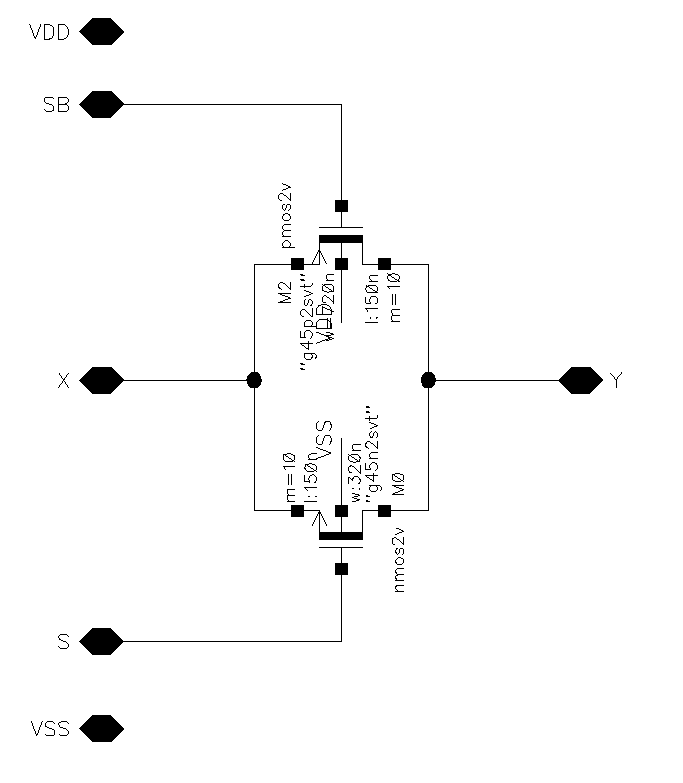
\includegraphics[width=2in]{images/sch_tg.eps}
		\caption{Transmission gate schematic, used to create normally open and normally closed switches alongside an inverter for appropriate clocking.}\label{fig:tg}
\end{figure}

\begin{figure}[htbp!]
		\centering
		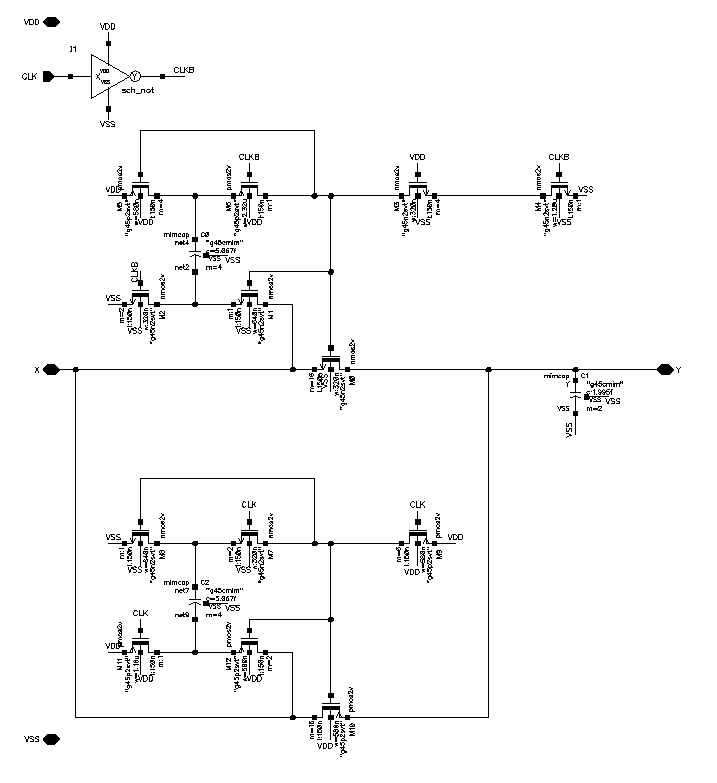
\includegraphics[width=4in]{images/sch_bootsw.eps}
		\caption{Bootstrapped switch schematic.}\label{fig:boot}
\end{figure}

The switched capacitor schematic created for this design is done such that each unit capacitor receives its own SPDT switch for connecting to either \(VSS\) for \(V_{bus}\), to provide consistency in the RC constant across the capacitor array and provide equal drive strength to each capacitor, and for ease of layout through having unit cells for placement.

\subsection{Comparator}

The comparator used in this design is the same rail-to-rail StrongARM comparator used in the previous flash ADC design. The schematic has been updated for simulation purposes to change any device finger definitions to strictly multiplier values for a hopefully better approximation of its behavior across monte carlo simulation, as shown in \cref{fig:comp_sch}. Its performance as extracted from layout and simulated at \qty{1.1}{\GHz} is shown in \cref{tab:comp_perf} for reference.

\begin{figure}[htbp!]
		\centering
	    \includegraphics[width=\textwidth]{images/sch_comp_sar.eps}
		\caption{RTR StrongARM comparator schematic with associated SR latch output to avoid invalid outputs.}\label{fig:comp_sch}
\end{figure}

\begin{table}[htbp!]
    \centering
    \begin{tabular}{ccc}
    \toprule
        Parameter & Units & Nominal \\
    \midrule
        Hysteresis & mV & 14.64 \\
        Prop. Delay (\qty{1}{\pF}) & ns & 1.5778 \\
        Prop. Delay (\qty{1}{\fF}) & ps & 414.07 \\
        DC Current & nA & 1.2868 \\
        W/decision & pW & 1.067 \\
        Layout Area & \(\qty{}{\um^2}\) & 119.79 \\
    \bottomrule
        
    \end{tabular}
    \caption{Comparator performance with extracted parasitics from layout.}\label{tab:comp_perf}
\end{table}

It is seen in the design of the flash ADC that this comparator design, while having merit for its ability to process a wide range of input signals, the extra devices on the input allow for a lot of kickback noise to be generated. The same kickback reduction scheme is employed in this design, where a transmission gate is placed after the local clock buffer to couple with the parasitic capacitance on the clock line and slow down the charging and discharging of the internal nodes \(V_A\) and \(V_P\), which reduces the current sent back through the inputs through the relationship in \cref{eq:kickback}. The resistance is increased to make up for coupling with the parasitic capacitance of only one comparator by increasing the length of the devices to \qty{1.2}{\um} total, as can be seen in the top right of \cref{fig:sar_sch}.

\begin{equation}
    I_{kickback} = -\left(\frac{2}{3}W\,L\,C_{ox} + C_{GS_{tot}}\frac{dV_A(t)}{dt} - C_{GS_{tot}}\frac{dV_P(t)}{dt}\right)\label{eq:kickback}
\end{equation}

Initially, no matter how small the RC time constant was made for charging the capacitor array, the comparator would still evaluate too early and contribute to massive DNL and INL due to its synchronous nature to the switching of the capacitor circuit. Methods of delaying the clock line to the comparator were investigated to hold off its evaluation until the nodes settled, but achieving the amount of delay needed at a clock frequency of only \qty{12}{\MHz} proved difficult without a polyphasic clock or other methods such as a PLL\@. A simple, but rather brute-force, solution was to invert the clock being sent to the comparator, so that it would evaluate half a cycle later and give the capacitors more than enough time to settle. If more time were to be given to this design, it may be desirable to implement a comparator driver within the Verilog controller, with some combinational logic to generate a clock cycle only when the ADC bits are being cycled. This would both increase power savings and reduce the amount of kickback noise generate during the critical sample and hold phase.

\subsection{Top-Level}

The top-level design for the SAR ADC is shown in \cref{fig:sar_sch}. The switched capacitor array is in the center, with the iterated instance naming schema shown. The multiplier value of 1 is visible for each instance; a schematic using multiplier values instead of iterated instances was also created for running PVT corners, since the simulation global PVT variations would not be greatly impacted by simplifying the simulation by multiplying the currents experienced by the instance according to its multiplier. The schematic using iterated instances was run for monte carlo simulation since this would yield better and more realistic results instead of having every device within the instance have 100\% correlation. The dynamic comparator is shown on the right with its ``asynchrobatic drive'' kickback-reduction circuitry, and the bootstrapped switches are on the left. A single bootstrapped switch instance was created for normally-open operation, and an inverter is placed before the input side reference switch to create normally-closed operation and better ensure the proper timing. The Verilog functional controller block is shown on the bottom.

\begin{figure}[htbp!]
		\centering
	    \includegraphics[width=\textwidth]{images/sch_sar.eps}
		\caption{Top level schematic of SAR ADC\@. Iterated instances of switched capacitor array are shown.}\label{fig:sar_sch}
\end{figure}

\section{Schematic Level Simulations}

PVT corner simulations are performed using tt, ss, sf, fs, and ff process corners, \(VDD\) of 1.8, 2.0, and \qty{2.2}{V}, and temperatures of 0, 40, and \qty{85}{\degree\C}. 1024 samples are chosen to give a minimum DNL and INL evaluation precision of \qty{0.25}{LSB}; while this does not give an accurate quantification of the true ADC performance, it is enough resolution to qualify the performance of the ADC against specifications while maintaining reasonable simulation time with the great number of internal nodes subject to switching and charge redistribution that must be evaluated. Monte carlo analysis is performed over a finite 100 points instead of a greater number for the same time constraint with this complex design. The standard monte carlo method is used with low-discrepancy sequence sampling for improved efficiency. A ``nullmfactorcorrelation=yes'' netlist option is included with the hope of Spectre properly interpreting this option and setting the correlation for any devices using a multiplier to 0\% instead of 100\%. A brief comparison showed that this was not the case, indicating that the gpdk045\_v5.0 models may not interpret this properly even though it was accepted in the netlisting logs.

The configuration management functionality provided by ADE Assembler is used during this design to perform behavioral simulations of the schematic prior to implementing instances using the gpdk045 components. Additional schematics for all components are constructed using idealized components provided by the \emph{analogLib}, \emph{ahdlLib}, and \emph{basic} libraries within Cadence Virtuoso, which are included in \cref{app1}. This design methodology greatly simplifies the debugging process by allowing for single circuit elements such as non-ideal switches to be implemented and debugged with all other components functioning as expected, narrowing down the breadth of where issues may lie. Once all individual components are known to work for the design at the system level, the integration process can begin with reduced circuit debugging overhead. 

\subsection{Testbench}

The testbench used for all simulations is shown in \cref{fig:tb_sar}. On the left, the \emph{vdd\_inherit} and \emph{vss\_inherit} instances from the \emph{basic} library are used to ensure supply continuity between Specture and AMS\@. The digital outputs are each loaded with the specified \qty{1}{\pF} load capacitance through an iterated capacitor, and are attached to an ideal 8-bit DAC, which regenerates an analog signal from the ADC's output to perform histogram analysis on. A piecewise linear source is used as the input stimulus to provide a triangle wave with rise and fall times set to half the input period, for analysis of any nonlinearity introduced by comparator hysteresis or other charging effects from the rising versus falling input wave. Analysis of this design is performed with a reference voltage of \qty{1}{\V} even though the comparator is designed for and has been proven to handle rail-to-rail inputs, to provide a worst-case condition for any circuit element's contribution to nonlinearity through the halved \(V_{LSB}\) at \qty{3.922}{\mV} resulting from the reduced reference.

Coherent sampling theory is applied to the evaluation of this ADC design due to the use of histogram functions to determine DNL and INL\@. The input waveform period and simulation time are parameterized based on the desired number of samples to be taken \(N_{samp}\), the sampling period \(T_{samp}\), and the desired number of input wave periods \(M\) which shall be odd, prime, and not a factor of \(N_{samp}\) for \(T_{samp}\). This is accomplished using the design variables setup as shown in \cref{tab:des_var}, which provides ease of analysis in the ADE Assembler as well. The transient analysis stop time is defined as \texttt{VAR("Nsamp")*VAR("Tsamp")}. The histogram analysis is setup as shown in \cref{fig:maestro}.

\begin{figure}[htbp!]
		\centering
	    \includegraphics[width=\textwidth]{images/tb_sar.eps}
		\caption{Testbench schematic used for all SAR simulations.}\label{fig:tb_sar}
\end{figure}

\begin{table}[htbp!]
    \centering
    \begin{tabular}{ll}
    \toprule
    \textbf{Name} & \textbf{Value} \\
    \midrule
        \texttt{REF} & \texttt{1} \\
        \texttt{VDD} & \texttt{2} \\
        \texttt{Tclk} & \texttt{Tsamp/12} \\
        \texttt{Tsamp} & \texttt{1u} \\
        \texttt{fs} & \texttt{1/Tsamp} \\
        \texttt{Nsamp} & \texttt{1024}\qquad(varies) \\
        \texttt{Tin} & \texttt{(Nsamp*Tsamp)/M} \\
        \texttt{M} & \texttt{3} \\
    \bottomrule
    \end{tabular}
    \caption{Design variables as set up within ADE test.}\label{tab:des_var}
\end{table}

\begin{figure}[htbp!]
		\centering
	    \includegraphics[width=\textwidth]{images/maestro_setup.png}
		\caption{Histogram analysis setup.}\label{fig:maestro}
\end{figure}

\subsection{Simulator Setup}

Spectre X simulator is enabled for this design with the AX accuracy preset and AX parasitic optimization preset checked, though no extracted simulations are performed for this project. The AX preset has its own overrides for the simulation algorithm integration method and accuracy presets. MS options were originally enabled to select the controller instance as a digital block, but later disabled due to issues. The only modifications made to the simulation algorithm are enabling \emph{pivotdc} and \emph{dc\_pivot\_check} to assist the DC solution, and enabling \emph{rebuild\_matrix} to provide more consistency from one run to another. Due to the functional Verilog controller, the AMS simulator is selected and a Connect Rule/Connect Module Based Setup is used using the built-in ConnRules\_inhconn\_mid ruleset.

Required simulation time is greatly extended by the fast-discharging nodes of the dynamic comparator requiring increased precision from the simulator, with 54:\qty{33}{min} required for each PVT corner's transient simulation to evaluate with similar results from monte carlo simulation. 2 threads are allocated by recommendation from the job log files, which enabled queuing of 24 active parallel simulation and netlisting jobs possible on the 48-core computers with negligible increase to the simulation time for each individual analysis, alleviating some of the time overhead.

\subsection {Results \& Discussion}

This ADC design passes specification across all 45 PVT corners, with maximum DNL of \qty{250}{mLSB} and INL of \qty{500}{mLSB}. Many corners state an achieved DNL of \qty{0}{LSB} and INL of \qty{28.422}{fLSB}, which truly means <\qty{125}{mLSB} in both cases due to the 1024 samples used in simulation yielding 4 points per binary code. Still, the ADC performs admirably and is robust against environmental and process variation. These results are summarized in \cref{tab:pvt_results}. An example waveform showing the charging behavior of the internal nodes at the typical corner is shown in \cref{fig:typ_wave}. The current measurements are taken from the V\_VDD source for \(I_Q\) and \(I_{tran_{max}}\) and the V\_REF source for \(I_{REF}\), at an arbitrary settled point during the transient simulation. These values may not represent the same as would be found via DC simulation, but represent the average performance of the ADC while it is running.

\begin{table}[htbp!]
    \centering
    \begin{tabular}{lllllll}
    \toprule
        \textbf{Parameter} & \textbf{Units} & \textbf{Max} & \textbf{Min} & \textbf{Mean} & \textbf{Median} & \textbf{Std Dev}\\
    \midrule
        \(\mathrm{DNL_{max}}\) & mLSB & 250 & 0 & 61.111 & 0 & 107.44 \\
        INL & mLSB & 500 & \qty{28.422e-12}{} & 77.778 & \qty{28.422e-12}{} & 147.41 \\
        \(I_Q\) & nA & 122.2 & 1.827 & 36.17 & 23.28 & 35.69 \\
        \(I_{REF}\) & \qty{}{\nA} & 54.3 & 0.06146 & 0.01102 & 1.687 & 18.42\\
        \(I_{tran_{max}}\) & mA & 80.94 & 40.92 & 58.17 & 57.09 & 10.54\\
        W/conversion & pW & 134.4 & 54.19 & 83.57 & 78.94 &  23.94\\
    \bottomrule
    \end{tabular}
    \caption{Flash ADC performance results across PVT corners, with a precision of \qty{10}{mLSB} for DNL and INL measurements.}\label{tab:pvt_results}
\end{table}

\begin{figure}[htbp!]
		\centering
	    \includegraphics[width=\textwidth]{images/waveform_typ.eps}
		\caption{Waveforms of selected internal and external nodes for SAR ADC during the first valid evaluation at the typical corner.}\label{fig:typ_wave}
\end{figure}

Monte carlo simulation proved not as successful for this design, with a \qty{3}{\sig} yield of 41\% for DNL and 89\% for INL\@. These results are summarized in \cref{tab:mc_results} with histograms in \cref{fig:dnl_hist,fig:inl_hist}. Some preliminary investigation suggests that this is contributed by comparator offset, since minimizing the variation attributed to the input devices of the comparator does improve the yield results. Additionally, the poor performance of the ADC occurs when the input is at its lowest voltages as seen in \cref{fig:mc_bad}, where offset would contribute the most severely. Since offset was not characterized over monte carlo simulations during the evaluation of the comparator, it is conceivable that this may be a contributing factor to the experienced nonlinearity. Minimizing the effects here through comparator device size increases would not be advisable due to the increased kickback and slowed operation, so a switched feedback offset compensation scheme may be advisable due to the high gain of the comparator. Closed loop stability would need to be evaluated in this case. Other options may include a fully differential input design, which can alleviate many of the effects of offset and kickback, but a different switching scheme may be necessary to prevent doubling of the switched capacitor device counts.

As previously mentioned, these results were achieved with a reference voltage of \qty{1}{\V}. Reviewing the statistical analysis from the monte carlo simulations, the yield may also have been improved by reducing the magnitude of the mismatch effects with respect to the overall \(V_{LSB}\), since the median and standard deviation are relatively low compared to the mean value. Also of note, the k-sigma method for monte carlo simulation was also investigated, which uses statistical parameters to determine a pass or fail of yield spec within a confidence interval. With confidence set to 80\%, it attempted to populate about 600 simulation points but a majority faced simulation errors; the ones that ran produced a slightly better yield than from the raw 100 points.

\begin{table}[htbp!]
    \centering
    \begin{tabular}{llllll}
    \toprule
        \textbf{Parameter} & \textbf{Units} & \textbf{Max} & \textbf{Min} & \textbf{Mean} & \textbf{Std Dev} \\
    \midrule
        DNL & mLSB & 1000 & 0 & 402.5 & 212.89 \\
        INL & mLSB & 1000 & \qty{28.422e-12}{} & 485 & 240.53 \\
    \bottomrule
    \end{tabular}
    \caption{Results from 100 points of monte carlo mismatch simulation, with a precision of \qty{250}{mLSB}.}\label{tab:mc_results}
\end{table}

\begin{figure}[htbp!]
		\centering
	    \includegraphics[width=\textwidth]{images/DNL_mc_hist.pdf}
		\caption{DNL monte carlo histogram.}\label{fig:dnl_hist}
\end{figure}

\begin{figure}[htbp!]
		\centering
	    \includegraphics[width=\textwidth]{images/INL_mc_hist.pdf}
		\caption{INL monte carlo histogram.}\label{fig:inl_hist}
\end{figure}

\begin{figure}[htbp!]
		\centering
	    \includegraphics[width=\textwidth]{images/mc_bad.eps}
		\caption{Example of improper evaluation when input is at its lowest during monte carlo simulation.}\label{fig:mc_bad}
\end{figure}

\section{Layout Floorplan}

Full layout of the ADC design is not required for this project, but a preliminary floorplan using the device instances in Layout GXL is created and shown in \cref{fig:sar_floorplan}. The switched capacitor instances are common-centroided outwards from the center, with the comparator and bootstrapped switches placed near the center. The full layout size is \qty{226.57}{\um} wide by \qty{190.96}{\um} tall, for a total layout area of \qty{43,265}{\um\squared}. The unit switched-cap layout is shown in and the bootstrapped switch layout is shown in \cref{fig:swcap_floorplan,fig:bootsw_floorplan}.

\begin{figure}[htbp!]
		\centering
	    \includegraphics[width=\textwidth]{images/sar_floorplan.eps}
		\caption{Full SAR layout floorplan.}\label{fig:sar_floorplan}
\end{figure}

\begin{figure}[htbp!]
    \centering
    \includegraphics[width=3in]{images/swcap_floorplan.eps}
    \caption{Unit switched capacitor layout floorplan, with switches on the top and inverters on the bottom.}\label{fig:swcap_floorplan}
\end{figure}

\begin{figure}[htbp!]
    \centering
    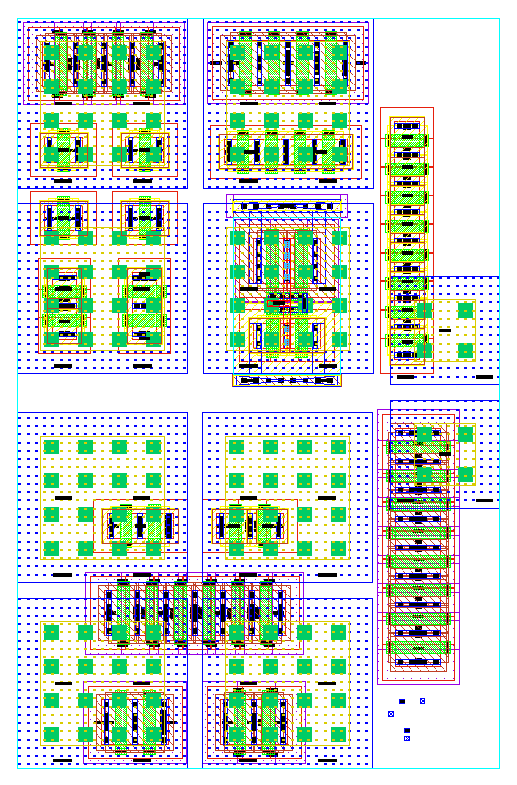
\includegraphics[width=3in]{images/bootsw_floorplan.eps}
    \caption{Bootstrapped switch layout floorplan. Switching devices are on the right underneath a small load capacitor for charge injection reduction.}\label{fig:bootsw_floorplan}
\end{figure}

\section{Conclusion}

This charge-redistribution based SAR ADC succeeds at meeting the design specifications across corners, and there is a clear path for increasing the \qty{3}{\sig} yield in monte carlo simulations, as the results achieved are workable but not ideal for fabrication as-is. The inclusion of this specific dynamic comparator design lends additional functionality, adaptability, and power savings through little DC current draw to this ADC design, while needing special consideration to not negatively impact the internal charge redistribution among the capacitors. An improved driving system has the potential for further improve the resolution of the ADC and allow for the reduction of necessary capacitor size.

\bibliographystyle{bib/IEEEtranDOI}
\bibliography{bib/export.bib}

\newpage

\renewcommand{\thesection}{A}
\section{Ideal Schematics}\label{app1}

\begin{figure}[htbp!]
    \centering
    \includegraphics[width=4in]{images/comp_ideal.eps}
    \caption{Behavioral comparator schematic.}\label{fig:comp_ideal}
\end{figure}

\begin{figure}[htbp!]
    \centering
    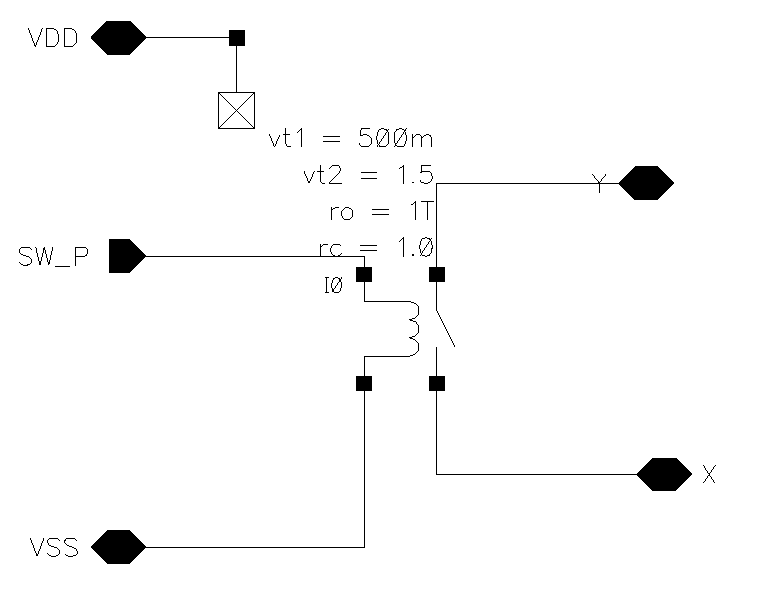
\includegraphics[width=4in]{images/no_ideal.eps}
    \caption{Behavioral normally-open switch schematic.}\label{fig:sw_no_ideal}
\end{figure}

\begin{figure}[htbp!]
    \centering
    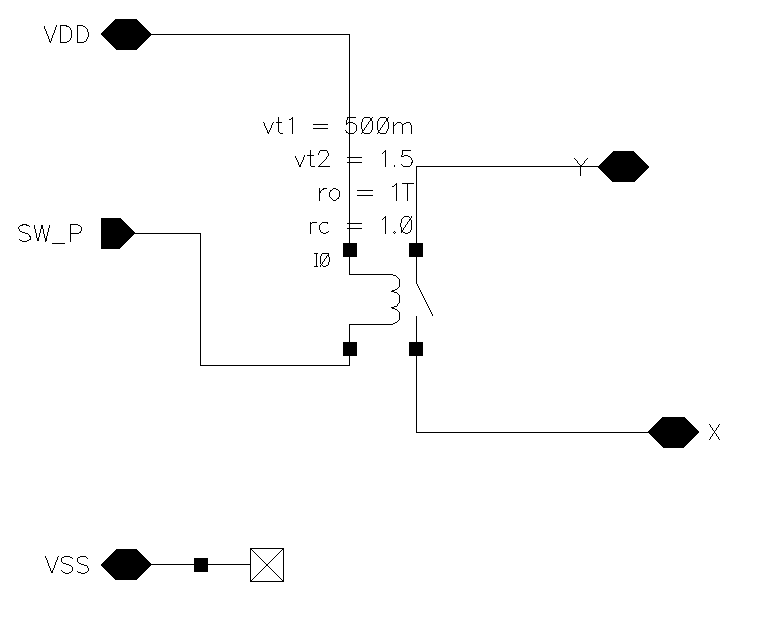
\includegraphics[width=4in]{images/nc_ideal.eps}
    \caption{Behavioral normally-closed switch schematic.}\label{fig:sw_nc_ideal}
\end{figure}

\end{document}